\subsection{Trigger and Data Acquisition}
\label{sec:tdaq}

During Run 2 operation between 2015--2018, the LHC delivered $pp$ collisions to ATLAS at instantaneous luminosities of
$10^{34}$\,cm$^{-2}$s$^{-1}$, at a bunch spacing of 25\,ns, giving 33.7 $pp$ interactions per bunch crossing on average
(see Figure~\ref{fig:int_lumi_multiyear}).
These values correspond to roughly $10^9$ $pp$ interactions per second.
It is not possible for the ATLAS detector and data storage facilities to both respond to and record every one of these interactions.
In fact, from a physics perspective it is not necssarily desirable to record every single interaction.
The vast majority of such interactions arise from uninteresting, soft collision processes which are not likely
to contain, for example, decays of Higgs bosons or of new particles not accounted for in the SM.
For this reason, the ATLAS detector employs an \textit{online}\footnote{The `online' environment refers to that of the
ATLAS detector during runtime. The `offline' environment refers to anytime in which the data being inspected
or analysed is not \textit{at that time} being recorded by ATLAS but instead has already been stored to permanent storage
and is readily accessible at any time.}
selection strategy to select potentially interesting candidate events to be further processed and considered
for permanent storage. This online selection strategy is referred to as the \textit{trigger} system~\cite{Jenni:616089}.

The ATLAS Run 2 trigger system consists of two levels: a hardware-based low-level
trigger, referred to as the \textit{Level-1} (L1) trigger, and a second level software-based high-level trigger (HLT)~\cite{PanduroVazquez:2244345}.
The L1 trigger uses relatively coarse-grained measurements from the calorimeters and MS.
It performs the first level of selection, reducing the initial input 40\,MHz rate of events by
accepting events at a maximal rate of 100\,kHz.
The L1 trigger performs searches for coarse proxies of interesting physics objects: leptons, photons, and jets.
It triggers on electrons and photons based on energy deposits in the EM calorimeter, limited to $\lvert \eta \rvert < 2.5$.
The hadronic calorimeter provides jet candidates to the L1 trigger system via calorimeter `towers' made up of
trigger elements constructed by a sliding window algorithm.
Each trigger element is constructed by calculating energy sums of calorimeter cells in $\eta - \phi$.
Muon-based L1 triggers are based on coincidences of hits along the layers of the MS that form
projective towers, or \textit{roads}, consistent with high-\pT~muons.

The candidate events selected by the L1 trigger system are forwarded to the HLT.
The HLT system is composed of a Level 2 (L2) trigger and the event filter (EF).
The L2 system is similar to the L1 trigger, but performs more refined measurements on the objects and
regions of the detector that resulted in the initial L1 trigger's decision to accept the event.
The EF is purely software based, using the ATLAS Athena reconstruction framework~\cite{AthenaRef}
to perform high level object reconstruction and identification using algorithms similar to those used
in the offline environment and described in Chapter~\ref{chap:objects}.
The HLT accept rate is roughly 1\,kHz.
The accepted events are sent to CERN's permanent storage facilities and are made ready for the offline analysis.
An overview of the trigger system is shown in Figure~\ref{fig:run2_trigger}.


\begin{figure}[!htb]
    \begin{center}
        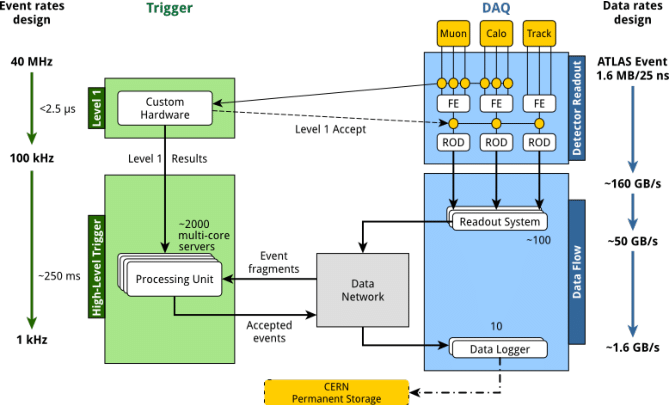
\includegraphics[width=0.7\textwidth]{figures/chapter2/tdaq/atlas_run2_trigger_system}
        \caption{
            Overview of the ATLAS Run 2 trigger and data-acquisition architecture.
            Data from the muon and calorimeter systems are used for the Level 1 (L1) trigger, reducing
            the input event rate from 40\,MHz to 100\,kHz.
            The data accepted by the L1 trigger are forwarded to the readout drivers (RODs)~\cite{Jenni:616089}
            which, among other things, re-shuffle the raw data into the standardized ATLAS event format~\cite{Bee:683741}.
            The events selected by the HLT at a rate of 1\,kHz are pulled from the RODs and then forwarded to the permanent
            storage.
            Figure taken from Ref.~\cite{PanduroVazquez:2244345}.
        }
        \label{fig:run2_trigger}
    \end{center}
\end{figure}
